%% ==============================================
%%           ANALYSIS AND DESIGN
%% ==============================================
%% Author: Fabian Sorn
%% ==============================================


\chapter{Analysis and Design of a Benchmark Framework}
\label{ch:analysisAndDesign}

In this chapter, we will further analyze the requirements of a benchmarking
framework, which allows users to benchmark specific charting operations. The
results of this analysis will then be combined with the results from the
previous two chapters for the design of our framework. First, we will have a
closer look at the two libraries, PyQtGraph and Matplotlib, which we will use
for the implementation of our use cases. Afterward, we will further analyze the
requirements for the use cases we have to be able to depict in the framework. In
the last section, we will then design the components as well as the main
functionality of it.


%% ==============================================
%%          Python Graph Libraries
%% ==============================================

\section{Python Graph Libraries}
\label{sec:application:libraries}

When benchmarking different Python Graph libraries, we will focus our attention
on two popular contenders for the implementation, which are very well accepted
in the scientific community.

\subsection{Matplotlib}
\label{sec:application:libraries:matplotlib}

Matplotlib is without a doubt the standard library for 2D data visualization in
Python. It offers publication quality visualization as well as an interactive
environment. The project was initialized by John D. Hunter as an easy to use
Python 2D plotting library, especially for users familiar with Data
Visualization in Matlab.
\cite{Matplotlib, MatplotlibHistory}

Matplotlib's central item is the \inlinecode{Python}{matplotlib.figure.Figure}.
The Figure itself does not yet display anything, neither a plot with axes nor
data. A plot is referred as an \inlinecode{Python}{matplotlib.axes.Axes}. A
figure can have multiple Axes in it. For each dimension in the data space, the
Axes contains \inlinecode{Python}{matplotlib.axis.Axis} objects, which
represent the minimum and maximum data limit for each dimension of the data. An
Axes object can be personalized through axis labels and a title. In Matplotlib
terminology, Artists are everything that is visible in a Figure. This includes
Labels, Lines and Bar Graphs, Axis Items and more. The last crucial component is
the Canvas, which is not really a visual component in the plot, but the
component responsible for rendering the image. A summary of all components can
be seen in \ref{a:fig:matplotlib:content}

Matplotlib is built for many different use cases. While showing data in
\gls{gui} applications is one of them, other use cases, like generating plots as
images for publications are possible as well. This is achieved by Matplotlib's
different backends. All available Backends can be divided into interactive and
hard copy ones. An example of an interactive backend is in our case PyQt5, but
other Frameworks like Tkinter or PyGTK are supported as well. Non-interactive
backends are for creating image files in different file formats like PNG, SVG,
PDF and more.
\cite{MatplotlibIntro, PythonDataVis}

Listing \ref{listing:application:matplotlib} shows the creation of a window
containing a plot representing a sinus curve through a line, a scatter plot and
a bar graph. For interaction, Matplotlib offers a toolbar, which lets you select
between different interaction modes like panning and zooming. As a backend
Matplotlib's Qt5 backend was used.  The resulting window can be seen in
Screenshot \ref{a:fig:matplotlib:window}.

\lstinputlisting[ 
    caption=Definition of a Window containing a plot created with Matplotlib,
    language=python,
    label=listing:application:matplotlib,
    firstline=4,
    lastline=32
]{resources/code/matplotlib_demo.py}

\subsection{PyQtGraph} \label{sec:application:libraries:pyqtgraph}

PyQtGraph is a pure python plotting library. Even though it does not offer as
many features as other Python plotting libraries like Matplotlib, PyQtGraph
promises much better performance. The project was initialized by Luke Campagnola
and is focused on providing plotting functionalities for engineering and science
applications. It provides simple plots containing line graphs, scatter plots,
bar graphs and more, but also image and video displaying, Region of Interest
widgets, 3D visualization and more.  Since our benchmarking efforts will be
tightly focusing on the collected use cases, we will restrict our usage of its
features mainly on two-dimensional plotting. PyQtGraph uses Qt's Graphics View
for drawing, which is a Framework for fast visualization of a large number of
custom 2D items. A big advantage it offers is a fast performance and the
possibility to interact and transform the scene through operations like
zooming or rotation.
\cite{GraphicsView}

Since PyQtGraph is built on top of Qt features, integrating it into Qt
applications is very simple. The central component for plotting is the
\inlinecode{Python}{pyqtgraph.PlotWidget}, which is derived from
\inlinecode{Python}{QtWidgets.QWidget}. When adding the plot widget to a
window, it comes with different components on the inside, as seen in
\ref{a:fig:pyqtgraph:content}. The central one is the
\inlinecode{Python}{pyqtgraph.PlotItem}, which is the actual plot. The widget
itself is only a wrapper for easy integration into Qt Applications. The plot
item contains different components of the plot, including a
\inlinecode{Python}{pyqtgraph.ViewBox}, the area data is visualized in,
a \inlinecode{Python}{pyqtgraph.AxisItem} representing the View Range
of the View Box, and a Title. Items that are actually representing a dataset are
added to the View Box. For this, PyQtGraph is offering different types of
representations like \inlinecode{Python}{pyqtgraph.PlotDataItem} for Scatter
Plots and Line Graphs and \inlinecode{Python}{pyqtgraph.BarGraphItem} for
representing data in a bar graphs.

Listing \ref{listing:application:pyqtgraph} shows the creation of a window
containing a plot representing a sinus curve in different ways. It displays the
same data sets in the same style as the Matplotlib example
\ref{sec:application:libraries:matplotlib}. The resulting window can be seen in
\ref{a:fig:pyqtgraph:window}.
\cite{PyQtGraphDoc}

\lstinputlisting[
    caption=Definition of a window containing a plot created with PyQtGraph,
    language=python,
    label=listing:application:pyqtgraph,
    firstline=2,
    lastline=25
]{resources/code/pyqtgraph_demo.py}


%% ==============================================
%%                   Analysis
%% ==============================================

\section{Analysis}
\label{sec:application:analysis}

After having a closer look at the two plotting libraries, this chapter will
focus on the analysis of the requirements which we will base the design and
implementation of our framework on.

Users interested in the performance of graph libraries often have a very clear
idea of what their use case looks like, since they already know the background
information of the data they want to plot. Because of this, the central
interface to the framework should be these use cases. Most higher level use
cases can be broken down in a simple operation or a sequence of operations. From
our collected use cases we can define the following requirements.

\begin{description}
    \item[Ease of Use] 
        The user should only define the relevant parts for his use cases.
        Everything else should be handled by the framework.
    \item[Widget and Operation]
        The central items for defining a use case are a widget, and an operation
        which is executed on this widget.
    \item[Multiple Use Cases]
        Adding and removing use cases has to be possible without much effort.
    \item[Parameterization]
        A use case has to be reusable for different parameters and has to be
        easily extensible.
    \item[Performance Expectations]
        The author has to be able to define his performance expectations per use
        case.
    \item[Timeout]
        In case a use case takes much longer than expect, it should be possible
        to define a timeout, which will terminate the use case's execution, if
        reached.
\end{description}

One framework type, which allows a very similar way of defining specific use
cases, are testing frameworks like unittest or pytest for python projects. Since
most users are to an extend familiar with their functionality, the interface
should conform the expectations built from the usage of these frameworks.

For easy execution of use cases, the framework will offer a command line
interface, which offers similar functionality as other python tools. The
\gls{cli} should conform the user's expectations in the same way with a few
additions specific to our needs. 

\begin{description}
    \item[Use Case Execution]
        Similar to frameworks like pytest, it should be able to execute multiple
        use cases as well as single ones.
    \item[Meaningful Results]
        After execution, the user should be able to clearly see the results of
        his use cases. This includes the use case, its performance requirements,
        the actually achieved performance and the parameters used in the run.
    \item[Profiling]
        Since Profiling introduces additional overhead to the code's execution,
        profiling should be optional and activatable through the \gls{cli}.
    \item[Profiling Visualization]
        Since profiles often contain large amount of data, they have to be
        visualized in a user friendly way.
\end{description}


%% ==============================================
%%                  Design
%% ==============================================

\section{Design}

\label{sec:application:design}

This section will focus on describing the design of the framework. The most
outer layer contains two components: the command line interface and the business
logic. The command line interface offers the user the possibility to start the
execution of his benchmarking use cases. Additionally it is responsible for
presenting the results after the execution finished. The second component is the
business logic, which is responsible for providing interfaces for defining use
cases, the logic for executing them, as well the functionality to record the
achieved results. We will refer to the executing part of the framework as the
launcher from now on.

\subsection{Benchmark Execution}

Figure \ref{fig:application:design:cli} shows the communication between the
user, the command line interface and the launcher when executing use cases from
the command line.  When the user starts the framework's executable, a \gls{cli}
instance is created, which parses the command line arguments and instantiates
the launcher. To keep the user interface exchangeable, launcher and \gls{cli}
are strictly separated from each other. The launcher will import the passed use
case modules, with which the initialization is completed. To start the
execution, the launcher offers a \inlinecode{Python}{run()} method. Each
collected use case will then be executed sequentially and its achieved results
collected. After all use cases are executed and all results are available, they
are passed back the \gls{cli}, where they can be presented to the user.

\begin{figure}[h]
    \centering
    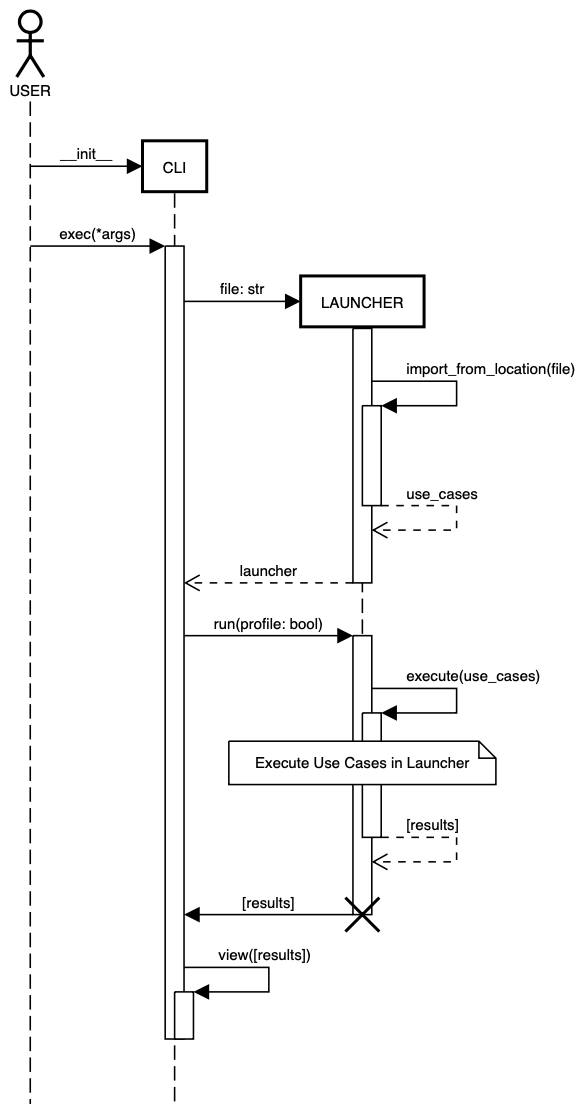
\includegraphics[width=11cm]{resources/img/sequence/cli}
    \caption{
        Sequence diagram showing the communication between the command line
        interface and the business logic.
    }
    \label{fig:application:design:cli}
\end{figure}


Next we will have a more detailed look at the inner workings of the launcher.
Its central task is the execution of use cases, which is visualized in depiction
\ref{fig:application:design:launcher}. Our goal is to allow executing a suite of
use cases similar to testing frameworks allowing the execution of entire test
suites at once. Each use case will have to be executed sequentially and in a
separate environment, to prevent different use cases having an influence on each
other.  The same principle applies to parameterized use cases. This means the
execution will take place in a nested loop with the outer one cycling through
the use cases and the inner one through its parameter combinations.

Visualization \ref{fig:application:design:launcher} introduces two new
components, which build the execution environment for a single use case. The
first component is the window, which will house our widget, on which we want to
operate. The second component is the executor, which is responsible for
executing the defined operation on the window and record timing information and
profiling statistics. After our Launcher is initialized and our benchmark files
are fully imported, we will execute each use case in all possible parameter
combinations. For each combination we create a new benchmarking window. The
window will then be passed to the executor. The executor will access all use
case related information and operations through this window reference. For
starting the execution, the executor offers a \inlinecode{Python}{run()}
function, which gets called by the launcher.

\begin{figure}[h]
    \centering
    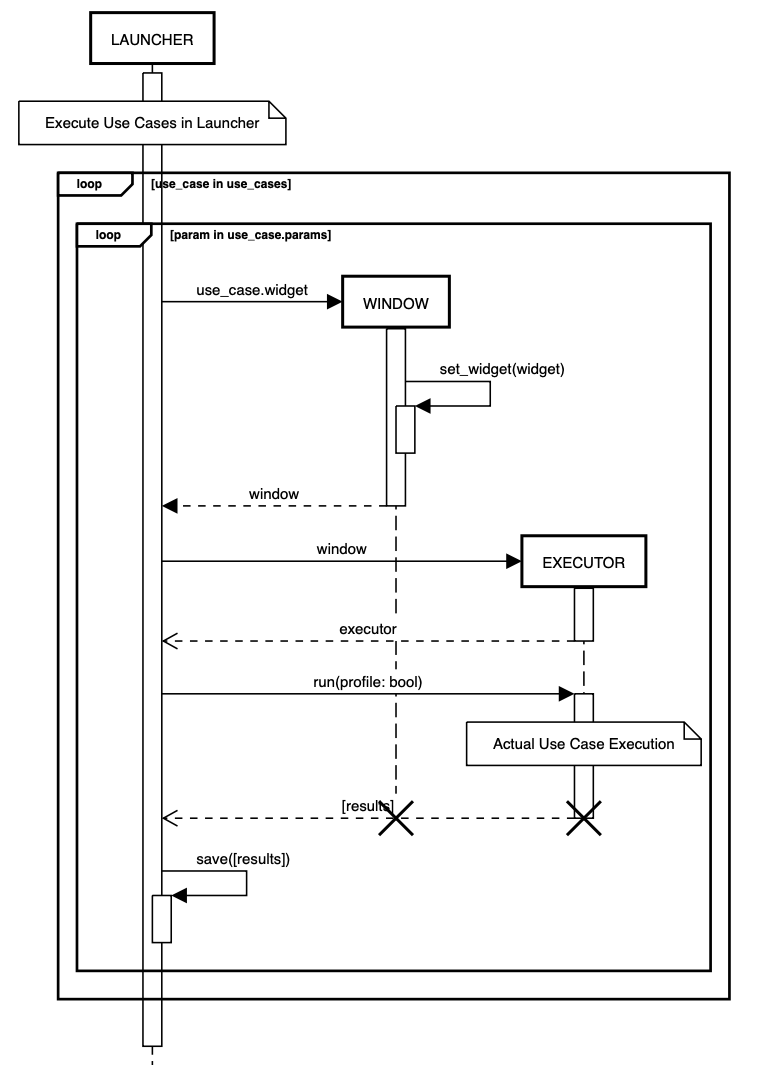
\includegraphics[width=12cm]{resources/img/sequence/launcher}
    \caption{
        Sequence diagram showing the execution of a set of use cases in more
        detail.
    }
    \label{fig:application:design:launcher}
\end{figure}

Depiction \ref{fig:application:design:executor} shows the execution of a single
use case in more detail. Before each operation, the current time stamp is taken.
If a profile is supposed to be created, the profiler is started right after
that.  Next the operation, which we want to benchmark, is executed on the passed
window reference. After it and all of its side effects are completed, the
profiler is stopped if necessary. Its statistics are added to the already
collected ones. This execution cycle is repeated, until the defined repeat count
or the timeout is reached. At the end, the timing information and the profiling
statistics will be returned to the launcher.

\begin{figure}[h]
    \centering
    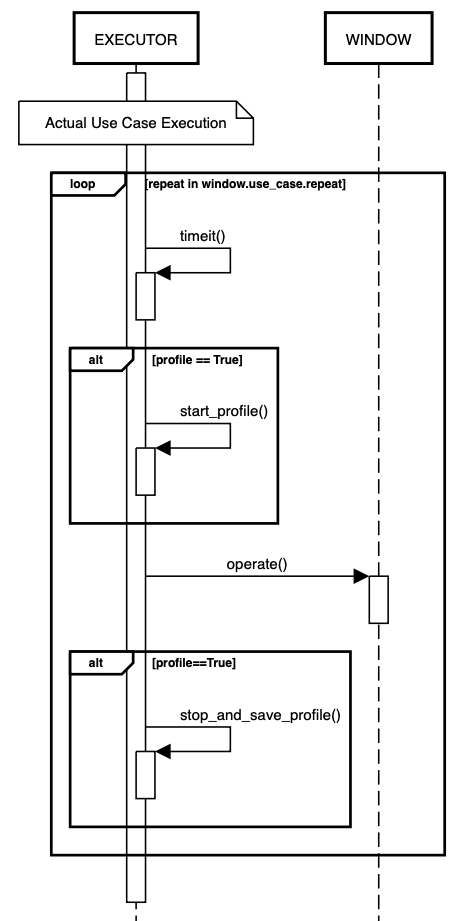
\includegraphics[width=8cm]{resources/img/sequence/executor}
    \caption{
        Sequence diagram showing the actual benchmarking execution on the window
        by the executor in more detail.
    }
    \label{fig:application:design:executor}
\end{figure}

Figure \ref{fig:application:design:classdiagram:widgetmark} shows a class
diagram of all classes involved in the sequence diagrams and their relationships
to each other. Additionally it shows the use case interface with all its
attributes and functions based on our analysis in section
\ref{sec:application:analysis}. To define a new use case, the user can subclass
this class and implement all necessary components. The results of a single use
case are represented by its own class, which can be passed between each of the
components involved in the execution until they can be display by the \gls{cli}.

\begin{figure}[h]
    \centering
    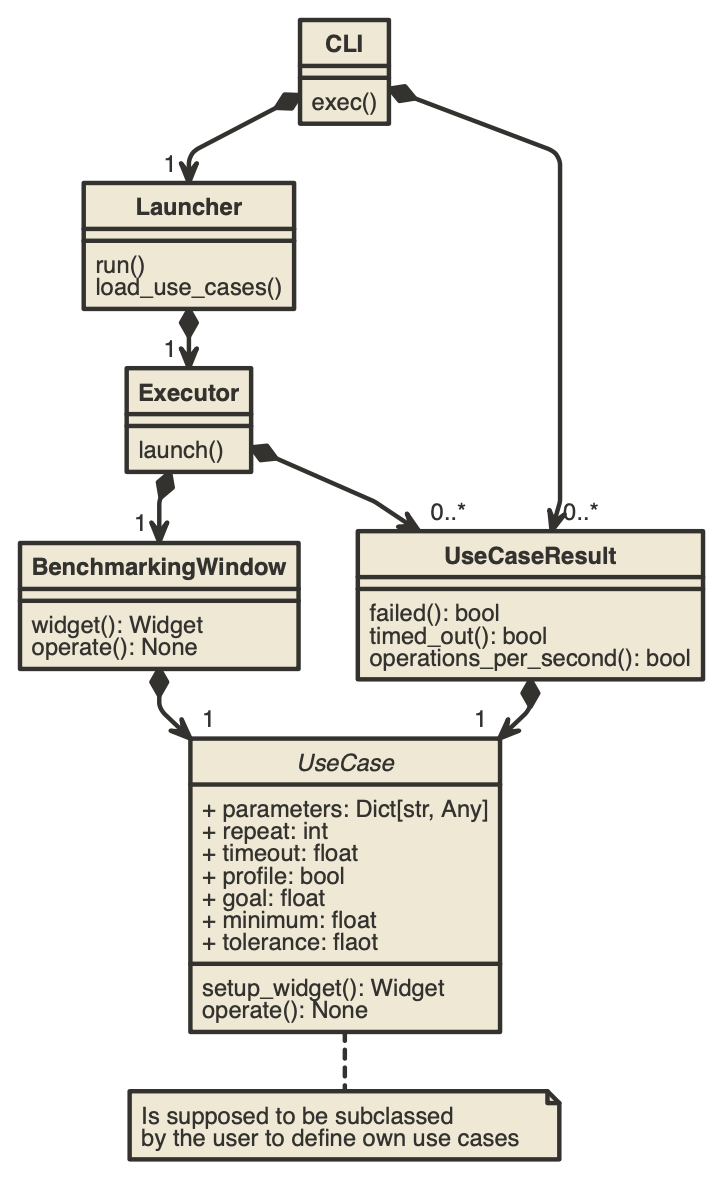
\includegraphics[width=8cm]{resources/img/class/widgetmark}
    \caption{
        Class diagram depicting all important classes involved in the
        Benchmarking Framework. 
    }
    \label{fig:application:design:classdiagram:widgetmark}
\end{figure}

\clearpage

\subsection{Use Case Definition and Plotting Abstraction Layer}

\label{sec:application:design:usecases}

In this section we will have a closer look at definition of use cases based on
the requirements collected in section \ref{sec:application:analysis}. A
single use case is represented by a class implementing the
\inlinecode{Python}{UseCase} interface. One python module can contain multiple
of these use case classes. By only executing classes derived from the use case
interface, we can allow defining other classes in the same modules as well
without them being executed by accident.

To define plotting benchmarks that are executable with different plotting
libraries we will define a unified interface for them. For the purpose of this
work, we will limit this interface to the functionality needed to execute our
use cases. In general this interface is limited to operations supported by all
graph libraries implementing it. With using the parameterization functionalities
of our use case interface, we can define higher level plotting benchmarks and
execute them using different libraries to compare the results from each of them.

\begin{figure}[h]
    \centering
    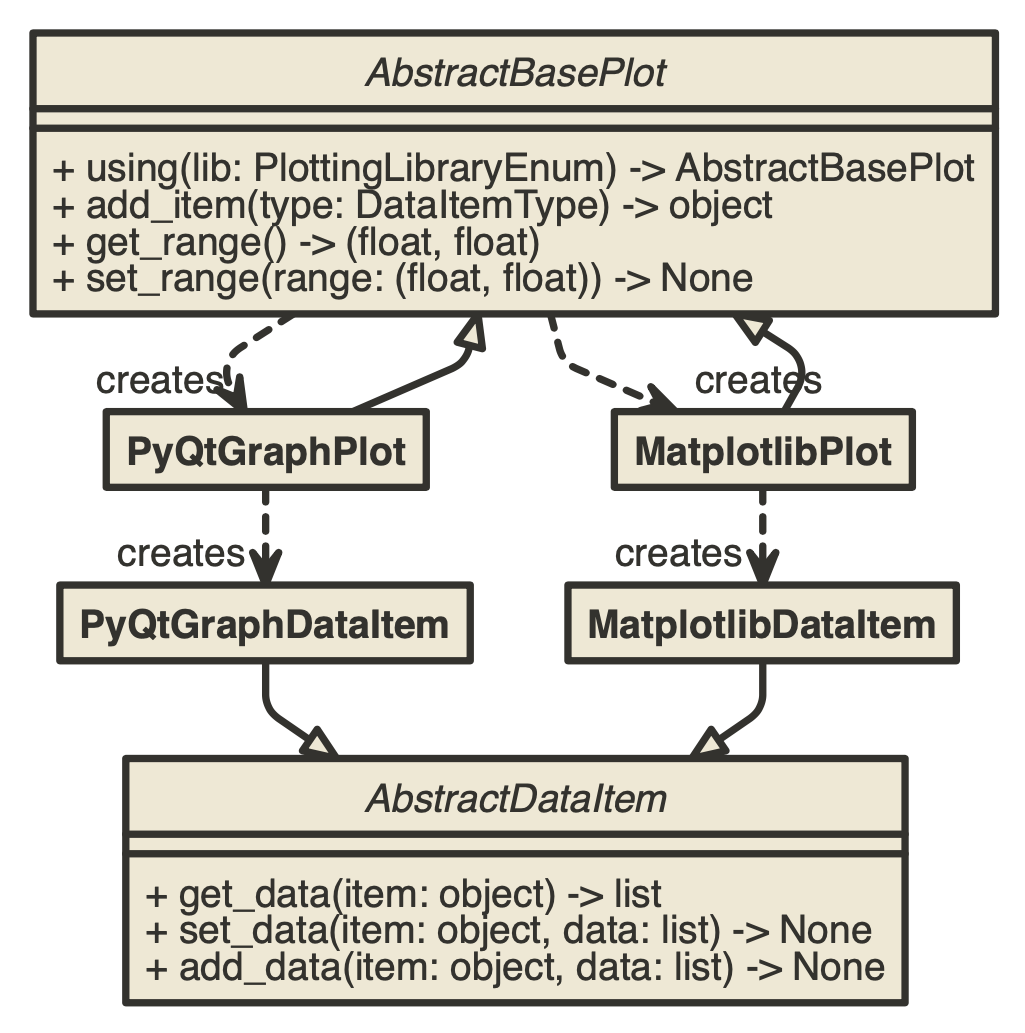
\includegraphics[width=7cm]{resources/img/class/plotabstraction}
    \caption{
        Class diagram depicting the plot abstraction interface and two
        subclasses for the python plotting libraries PyQtGraph and Matplotlib. 
    }
    \label{fig:application:design:classdiagram:plot}
\end{figure}

Figure \ref{fig:application:design:classdiagram:plot} shows the abstract base
classes for the plot widget as well as data items like curves, bar graphs,
scatter plots and more. The class \inlinecode{Python}{AbstractBasePlot} offers
plot functionalities to add a new item, get and set the current view range and a
factory method for creating a plot using a specific plotting library. The two
subclasses \inlinecode{Python}{PyQtGraphPlot} and
\inlinecode{Python}{MatplotlibPlot} can implement the functionality defined by
the base class using their specific \gls{api}. The
\inlinecode{Python}{AbstractDataItem} on the other hand defines a common
interface for setting, getting and adding new data to a data item of a plot.
Similar to the \inlinecode{Python}{AbstractBasePlot}, this interface is
implemented by the two subclasses \inlinecode{Python}{PyQtGraphDataItem} and
\inlinecode{Python}{MatplotlibDataItem} using their specific \gls{api}.

Listing \ref{listing:application:plotabstraction} shows, how the interface
should be usable in a standard Qt application. Which library is used for the
visualization can be controlled during the widget's initialization using the
\inlinecode{Python}{AbstractBasePlot} factory method
\inlinecode{Python}{using()}.

\lstinputlisting[ 
    caption=Creating a plot showing a sinus curve using the Plot Abtraction 
            Layer,
    language=python,
    label=listing:application:plotabstraction,
    firstline=9,
    lastline=30
]{resources/code/plot_abstraction.py}


\subsection{User Interface}

In this section we will have a look at the design of the command line interface
based on the requirements we collected in \ref{sec:application:analysis}. Since
our command line is supposed to be easily usable for users of other testing
frameworks, it should meet the user's expectations. The main purpose of the
command line is starting the execution of one or multiple use cases. Listing
\ref{listing:application:cliusage:location} shows how to specify, which use
cases should be executed. It should be possible to define a folder, a python
module or a specific use case inside a python module. For python modules
containing use cases, we will introduce a specific naming convention. The
default one should be, that the python module's name is prefixed with
\inlinecode{bash}{bench_}, similar to test files being often prefixed with
\inlinecode{Python}{test_}. This pattern should be configurable from the
command line as well.

\lstinputlisting[ 
    caption=Executing use cases from the command line,
    language=bash,
    label=listing:application:cliusage:location,
    lastline=39
]{resources/code/widgetmark_cli_usage.sh}

Additionally the command line should allow us to configure, if we want to run
the framework with or without profiling, as well as the location the files are
saved in. Listing \ref{listing:application:cliusage:profile} shows these
configuration options on the command line as well as the generated files.

\lstinputlisting[ 
    caption=Starting benchmarks and create profiles for them,
    language=bash,
    label=listing:application:cliusage:profile,
    firstline=40,
    lastline=52
]{resources/code/widgetmark_cli_usage.sh}

Additionally the \gls{cli} should provide a visualization option for the
profiling statistics. Simply printing the profiling statistics to the command
line would not be very helpful, since they can grow very fast in size. Because
of this, there are multiple tools available, which offer a much more user
friendly visualization. For our purposes we decide for \emph{snakeviz}, a
browser based graphical viewer for profiling files.  \cite{Snakeviz}

To improve the usability of the \gls{cli}, a help function should be offered
which explains what the framework is and how it is going to be used.
Listing \ref{listing:application:cliusage:help} shows how such a help message
could look like. Additionally it should be possible to run the \gls{cli} with
additional output when searching for bugs in a use cases definition. 

\lstinputlisting[ 
    caption=Starting benchmarks and create profiles for them,
    language=bash,
    label=listing:application:cliusage:help,
    firstline=58,
    lastline=68
]{resources/code/widgetmark_cli_usage.sh}

After the execution is completed, the \gls{cli} output should show all
important information about the found files, the use cases, the performance
requirements, the parameters and the actual reached frame rate. Listing
\ref{listing:application:cliusage:output} shows, how these informations could be
presented.

\lstinputlisting[ 
    caption=Output of the CLI with showing the benchmark results,
    language=bash,
    label=listing:application:cliusage:output,
    firstline=69,
]{resources/code/widgetmark_cli_usage.sh}

